\section{LayoutLMv3 kết hợp chữ, vị trí và ảnh}
\textcite{huang2022} đề xuất một Transformer tiếp nhận token văn bản và các ô ảnh. Tọa độ hai chiều giúp gắn token chữ với vị trí trên trang, còn các ô ảnh cung cấp thông tin thị giác. Quá trình tiền huấn luyện gồm khôi phục chữ bị che, dự đoán token ảnh bị che và dự đoán xem ô ảnh tương ứng với một từ có bị che hay không. Mục tiêu cuối hỗ trợ liên kết thông tin giữa chữ và ảnh.

\noindent\begin{minipage}{\textwidth}
\centering
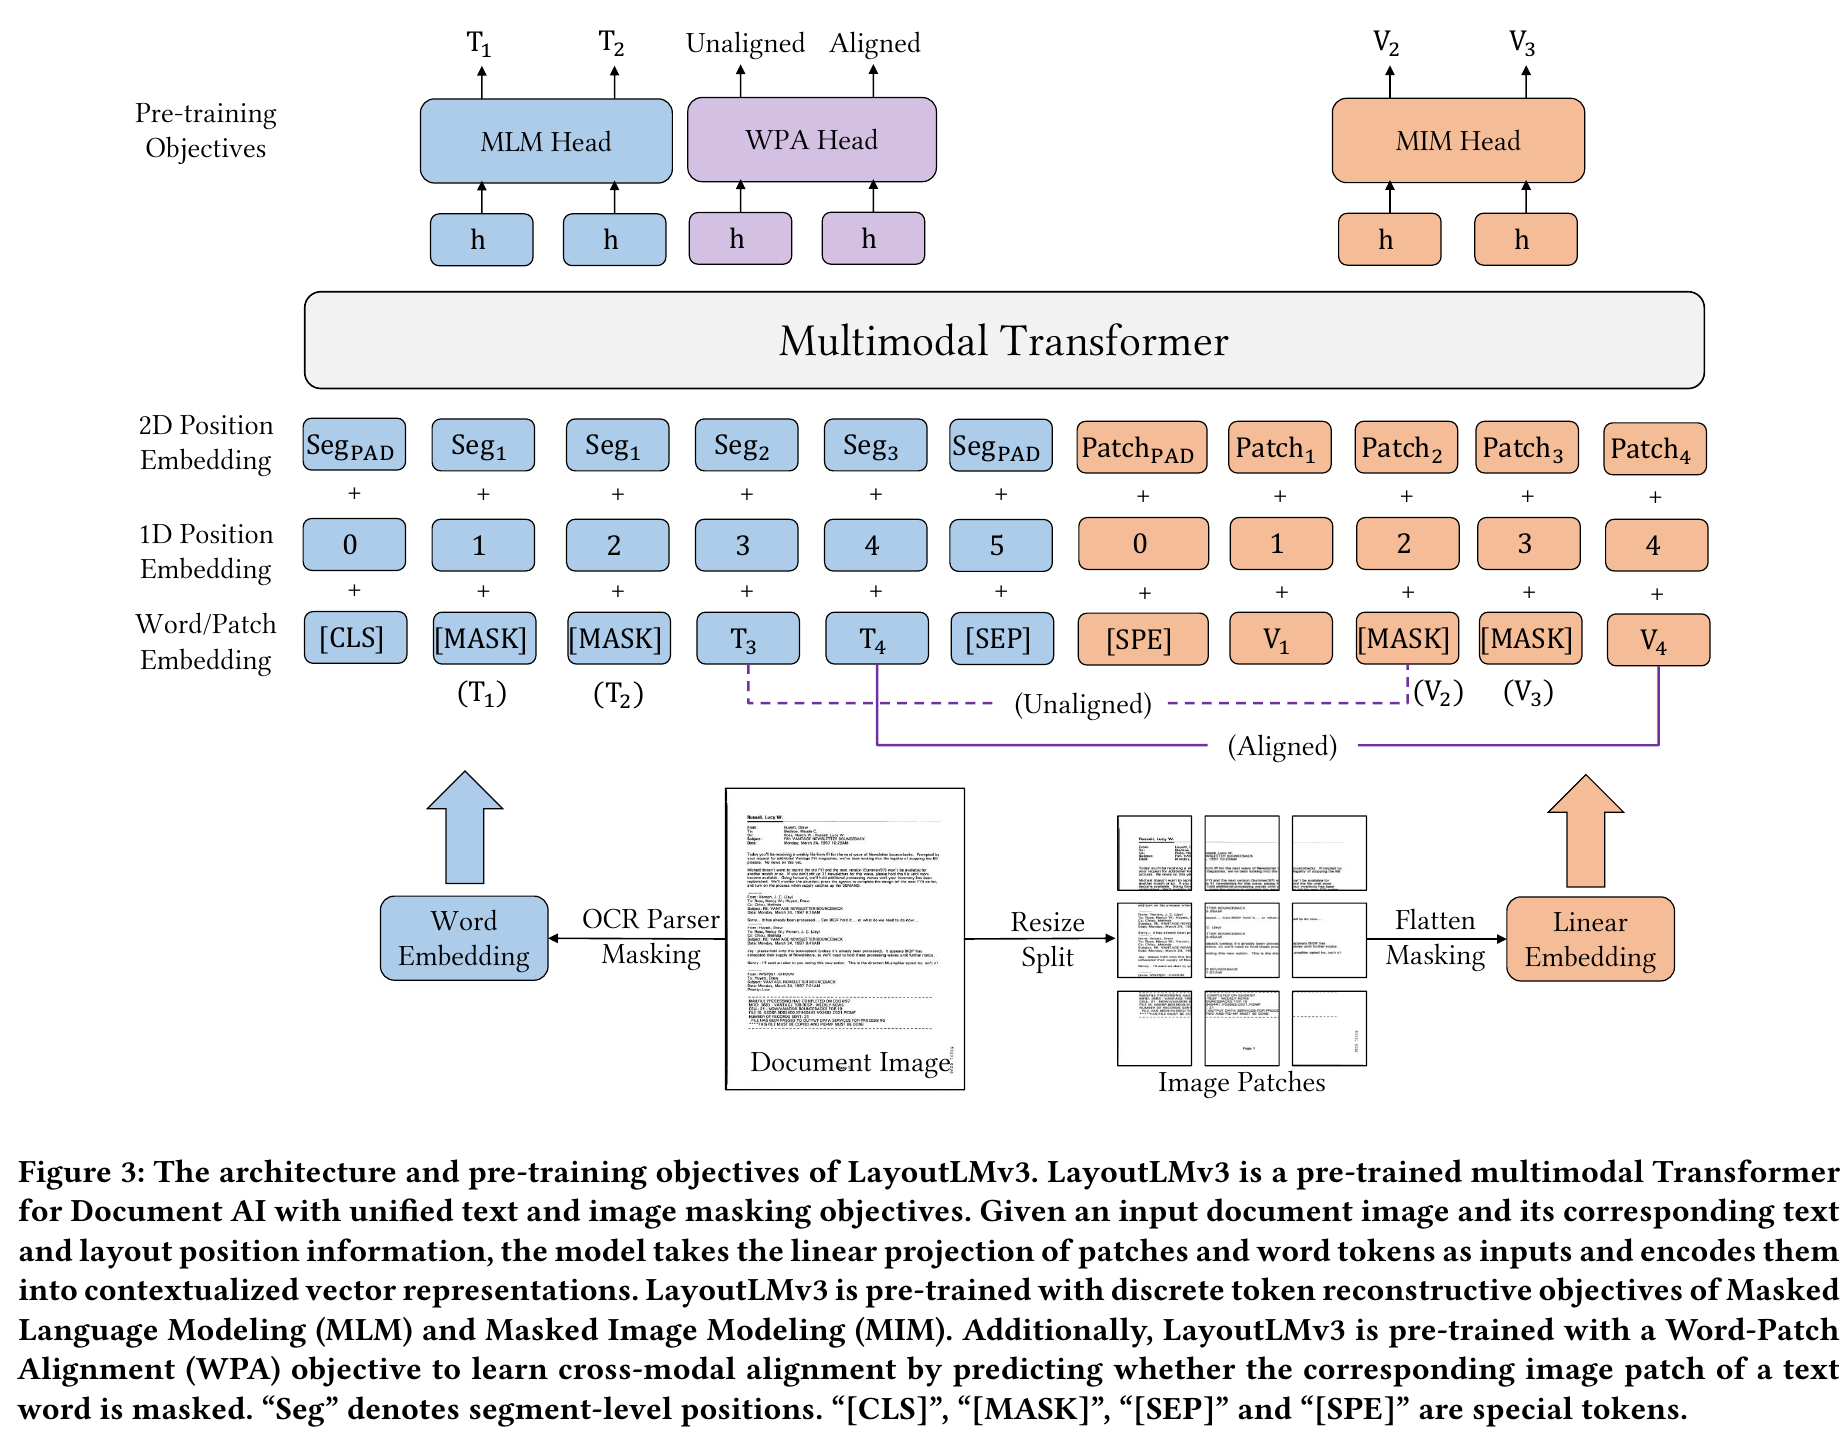
\includegraphics[width=0.94\textwidth,height=7cm,keepaspectratio]{picture/layoutlmv3-paper-figure-3.png}
\captionof{figure}{Các mục tiêu tiền huấn luyện của LayoutLMv3}
{\small (Nguồn: Hình 3 của \textcite{huang2022})\par}
\end{minipage}

Trong đề tài, nhóm nạp trọng số đã tiền huấn luyện và tinh chỉnh đầu phân loại token theo nhãn BIO. Đầu vào gồm ảnh và văn bản cùng tọa độ từ chú thích của bộ dữ liệu. Ba mục tiêu trong hình thuộc giai đoạn tiền huấn luyện của bài báo.

